\chapter{Introduction}\label{chap:introduction}
In past few years there has been a huge chatter about cloud computing. Every Organization in this era is at least reviewing or looking at resources to see if moving to cloud would same them time and efforts. Cloud as we are aware makes provisioning of new resources quickly so an organization can concentrate their efforts on tasks that create more value for them rather than concentrating their resources on procuring hardware or provisioning servers. At the same time companies do not want to invest in hardware that is hardly utilized for about 3-4 hours in a day thus making a classic case for moving to cloud. In cloud you utilize resources for the time you need and terminate the instance when your work is complete and paying only for the time a resource is up and utilized. 
\\

Businesses are often confused by the thought of moving to cloud. While they may have valid concerns, cloud supporters have advantages to show , but ultimately it is the business who has to decide if the advantages outweigh their concerns.\cite{MTechLabs}
\begin{figure}[!htb]
    \center{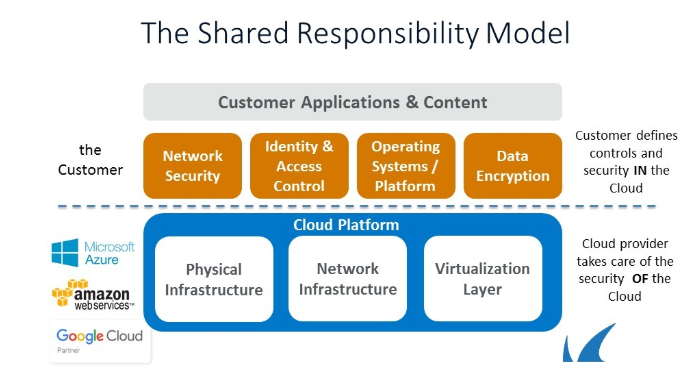
\includegraphics[width=\textwidth]
    {figures/experiments/Shared_Responsibility_Model.png}}
    \caption{\label{fig:shared_responsibility_model} Shared responsibility model}\cite{SecurityModel}
\end{figure}
%\begin{center}
%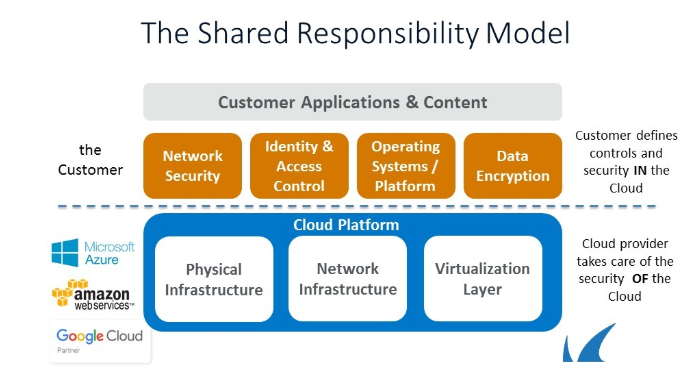
\includegraphics[scale=0.75]{figures/experiments/Shared_Responsibility_Model.png}
%\end{center}

\section{Concerns}
Concerns  and what do cloud supporters have to say about them : 


\subsection{Security}
Cloud environments experience – at a high level – the same threats as traditional data center environments, the threat picture is the same. Both run softwares, softwares have vulnerabilities, and there is someone out there waiting to exploit these vulnerabilities. However security on cloud is a shared responsibility model of security. While cloud provider takes care of the security of the cloud , some aspects of security remain sole responsibility of the consumer. Effective cloud security depends on knowing and meeting these consumer responsibilities. 

\subsection{Data Privacy} 
Cloud computing involves the dispersal of data across servers located anywhere in the world. Like globalization of networks. By crossing borders, involves considering countries with restrictive privacy and protection laws . This is somewhat covered as part of customer responsibility towards cloud security. For this corporations need to understand what kind of data will they load into cloud and who will have access to this data. \cite{DataPrivacy}

Other aspect of data privacy is handling sensitive data. Yes one of the problems is that this technology is light years ahead of the law and there are questions that need to be answered. Who owns the data, consumer or the hosting cloud provider? Can a cloud deny the consumer access to their own data or can it share this data with marketing firms  Obviously , the safest approach is data privacy is more a consumer responsibility. Keep data under proper control and apply data encryption methods. Regarding the question about laws, each company wants to protect their reputation. To get more clients and maintain them, cloud providers would uphold your data privacy. There are getting more managed and include all the necessary provisions that one should take while setting up their data on cloud. \cite{DataPrivacy2}

\subsection{ROI}
ROI or Return of Investment is widely a measure of financial success and can be a measured in a variety of ways. If you move to public cloud, you generally decrease invenstment but increase cost. With private cloud, it is vice-versa. But what matters is value to business, customer value, seller value, market brand value, corporate value. In case of cloud services, these relate to productivity, speed, size and quality. \cite{ROI}

\subsection{Implementation Cost}  
There are a number of challenges in figuring out the implementation cost for the cloud. Recently FASB has come out with accounting procedures on how to evaluate cloud costs.

\subsection{Integration Issues} 
Most enterprises would apply an incremental model of implementation. It is less risky than big-bang. This requires integration of services.The risk of not being able to integrate is critical. If you cannot build a system, you cannot use it. This also adds to the cost of including glue-softwares to connect various interfaces .It could involve rewrite of code or existing process models. Not to forget significant skills are required to assemble and customize multiple cloud services , requiring the applications to be loosely coupled, programmed to perform in an integration layer instead of underlying infrastructure.  

\subsection{System Quality}  
\begin{itemize}
	\item Performance 
	\item Functionality 
	\item Manageability 
	\item User satisfaction 
\end{itemize}

\subsection{Resource Comparisions}

\subsubsection{Storage}

\begin{longtable}{p{3.7cm}|p{3.7cm}|p{3.7cm}}
\caption{Storage characteristics \label{table:storage_char}}\\

% This is the header for the first page of the table
\hline
\hline
{\textbf{Storage Features}} &
{\textbf{S3}} &
{\textbf{GCloud}}\\
\hline
\endfirsthead

%This is the header for the remaining page(s) of the table...

\multicolumn{3}{c}{{\tablename} \thetable{} -- Continued} \\[0.5ex]
\hline
\hline
{\textbf{Storage Features}} &
{\textbf{S3}} &
{\textbf{GCloud}}\\
\hline
\endhead

%This is the footer for all pages except the last page of the table...
\multicolumn{3}{l}{{Continued on Next Page\ldots}} \\
\endfoot

%This is the footer for the last page of the table...

\hline \hline
\endlastfoot

%Now the data...

{Durability} & {99.999999999\%} & {99.999999999\%} \\ % inserting body of the table
\hline
{Availability} & {data is automatically distributed across minimum of 3 physical Azs( 57 Azs across 19 geographic regions )} & {99.9\% SLA for regional and 99.95\% SLA for multi-regional} \\
\hline
{Scalability} & {Maximum size limit of 5TB. Largest object uploaded in single PUT is 5GB. Objects > 100MB, should be uploaded via multipart upload capability} & {Maximum size limit of 5TB. Objects > 5MB should be uploaded via multipart or resumable uploading} \\
\hline
{Costs} & {Pricing based on data storage levels, based on frequency of access, size of data. Pricing model varies as per size tier. PUT, COPY , etc. operations are priced for frequent and infrequent access per 1000 transactions  as well as for retrieval from archive.} & {Pricing model is different for different regions, frequency of access and size of data. PUT, COPY , GET operations are priced per 10000 transactions. It does have minimum days of storage and charges penalties for early deletion for cold storage} \\
\hline
{Security} & {Supports 3 different forms of encryption. Supports security standards} & {Encryption is automatic and no customer action is required. More than 1 encryption mechanisms used.} \\ 
\hline
{Compliance} & {Consumer retains complete control and ownership over the region in which their data is physically located, making it easy to meet regional compliance requirements. Compliance certifications, including PCI-DSS, HIPAA/HITECH, FedRamp, EU Data Protection Directive, FISMA, etc.} & {Compliance certifications include PCI-DSS, HIPAA/HITECH, SOC* , FedRamp, GDPR,  etc.}\\
\hline
{Query in place} & {Allows to run sophisticated Big Data analytics on your data w/o moving the data into a separate analytics system} & {Allows to run Big Data analytics on data ( Big Query )} \\
\hline
{Flexible Management} & {Storage administrators can classify, report and visualize data usage trends to reduce costs and improve service levels. Objects can be tagged based on their features to control storage consumption, cost and security} & {Pricing modes based on different regions . Does not offer volume discounts} \\

\end{longtable}

\begin{longtable}{p{3.7cm}|p{3.7cm}|p{3.7cm}}
\caption{Server Based Compute \label{table:compute}}\\

% This is the header for the first page of the table
\hline
\hline
{\textbf{Server Based Computing}} &
{\textbf{AWS EC2}} &
{\textbf{Google Compute Engine}}\\
\hline
\endfirsthead

%This is the header for the remaining page(s) of the table...

\multicolumn{3}{c}{{\tablename} \thetable{} -- Continued} \\[0.5ex]
\hline
\hline
{\textbf{Server Based Computing}} &
{\textbf{AWS EC2}} &
{\textbf{Google Compute Engine}}\\
\hline
\endhead

%This is the footer for all pages except the last page of the table...
\multicolumn{3}{l}{{Continued on Next Page\ldots}} \\
\endfoot

%This is the footer for the last page of the table...

\hline \hline
\endlastfoot

%Now the data...

{Elastic web-scale computing} & {enables to increase/decrease capacity within minutes with the additional feature of auto scaling} & {managed instances can be set up for auto-scaling} \\ % inserting body of the table
\hline
{Completely controlled} & {consumer has complete control over instances including root access} & {consumer has complete control of systems and unlimited flexibility} \\
\hline
{Flexible cloud hosting services} & {variety of instance shapes available} & {variety of instance shapes available} \\
\hline
{Integrated} & {integrated with multiple Google services to provide end to end cloud solution} & {integrated with multiple Google services to provide end to end cloud solution} \\
\hline
{Reliable} & {The Amazon EC2 Service Level Agreement commitment is 99.99\% availability for each Amazon EC2 Region.} & {Google cmpute engine guarantees 99.99\%  monthly uptime percentage to customers} \\ 
\hline
{Secure} & {Amazon EC2 works in conjunction with Amazon VPC to provide security and robust networking functionality for your compute resources} & {Google Compute Engine has ISO 27001, SOC 1, SOC 2, SOC 3, SSAE-16 certifications, exhibiting  commitment to information security}\\
\hline
{inexpensive} & {pay for what you use. Various options available to reduce cost for low risk or less available operations requirements( ex- spot instances )} & {after a 10 min minimum charge, pay for what you use} \\
\hline
{Easy to start} & {Free to start} & {Free to start} \\

\end{longtable}


\begin{table}[ht]
\caption{Serverless Compute} % title of Table
\centering % used for centering table
\begin{tabular}{>{\centering\arraybackslash}m{3.7cm}|>{\centering\arraybackslash}m{3.7cm}|>{\centering\arraybackslash}m{3.7cm}} % left justified columns (3 columns)
\hline\hline %inserts double horizontal lines
Serverless Compute & AWS Lambda & Google Cloud Function \\ [0.5ex] % inserts table
\hline % inserts single horizontal line
No Server Management & Automatically runs your code w/o requiring to provision or manage servers. & code executes in fully managed environment, no need to provision any infrastructure or worry about managing any servers \\ % inserting body of the table
\hline
Continuous Scaling & auto-scaling enabled & auto-scaling enabled \\
\hline
Pricing & charged for every 100 ms of code execution & charged for the time code runs \\
\hline
Portable & supports Node.js, python , C\# and Go & can be written in Node.js or python making them portable \\ [1ex] % [1ex] adds vertical space
\hline %inserts single line
\end{tabular}
\label{table:nonlin} % is used to refer this table in the text
\end{table}